\documentclass{article}
\usepackage{amsmath,amssymb}
\usepackage{graphicx}
\usepackage{float}

\title{Malaria Transmission Dynamics with Mosquito Treatment: Reproduction Number Analysis}
\author{Yaghoub Shahmari}
\date{\today}

\begin{document}

\maketitle

\section{Closed-Form Expression for the Basic Reproduction Number, \(R_0\)}

When the system is linearized about the disease-free equilibrium (DFE), we set 
\[
I_H=E_{1M}=E_{2M}=I_M=E_{1T}=E_{2T}=I_T=0,
\]
and the human population is entirely susceptible, i.e. \(S_H=1\). For the mosquito population, we assume that the total population is normalized:
\[
S_M+S_T=1.
\]
In the mosquito subsystem the DFE is obtained by solving the linear system:
\[
\begin{pmatrix}
-(t+g)& h\\[1mm]
t & -(h+g)
\end{pmatrix}
\begin{pmatrix}
S_M^*\\[1mm]
S_T^*
\end{pmatrix}
=
\begin{pmatrix}
- g\\[1mm]
0
\end{pmatrix}.
\]
A short calculation yields
\[
S_M^*=\frac{h+g}{t+h+g},\quad
S_T^*=\frac{t}{t+h+g}.
\]

Next, following the standard next-generation approach the infection cycle is “completed” by tracking the passage from an infectious human to an infected mosquito and back to a newly infected human.

\subsection*{Untreated Branch}
An infectious human infects a mosquito (via a bite) at rate \(ac\). In the untreated branch, the infection passes sequentially through two latent stages:
\[
\begin{aligned}
E_{1M}&=\frac{ac\,S_M^*}{t+s_{1M}+g}\,I_H,\\[1mm]
E_{2M}&=\frac{s_{1M}}{s_{2M}+g}\,E_{1M},\\[1mm]
I_M&=\frac{s_{2M}}{g}\,E_{2M}.
\end{aligned}
\]
Thus the passage (or survival) probability for the untreated branch is
\[
\pi_M=\frac{ac\,S_M^*}{t+s_{1M}+g}\cdot\frac{s_{1M}}{s_{2M}+g}\cdot\frac{s_{2M}}{g}.
\]

\subsection*{Treated Branch}
Similarly, the treated branch follows:
\[
\begin{aligned}
E_{1T}&=\frac{ac\,S_T^*}{s_{1T}+g}\,I_H,\\[1mm]
E_{2T}&=\frac{s_{1T}}{s_{2T}+g}\,E_{1T},\\[1mm]
I_T&=\frac{s_{2T}}{g}\,E_{2T},
\end{aligned}
\]
with passage probability
\[
\pi_T=\frac{ac\,S_T^*}{s_{1T}+g}\cdot\frac{s_{1T}}{s_{2T}+g}\cdot\frac{s_{2T}}{g}.
\]

\subsection*{Additional Contribution: Untreated Mosquitoes Receiving Treatment During Latency}
Experimental evidence (see slide~10) indicates that some mosquitoes in the untreated branch are treated during the latent period. Their contribution is given by:
\[
\pi_{extra}=\frac{ac\,S_M^*}{t+s_{1M}+g}\cdot\frac{t}{t+s_{1M}+g}\cdot\frac{s_{1T}}{s_{1T}+g}\cdot\frac{s_{2T}}{s_{2T}+g}.
\]

\subsection*{Overall Expression for \(R_0\)}
An infectious human transmits to mosquitoes (at rate \(ac\)) and, in turn, an infectious mosquito transmits to humans at rate \(ab\). With the mosquito-to-human ratio \(m\) and the human recovery rate \(r\), the total number of secondary human infections produced by one infected human is
\[
R_0=\frac{m\,a\,b}{r}\Bigl[\pi_M+\pi_T+\pi_{extra}\Bigr].
\]
Substituting the expressions for \(\pi_M\), \(\pi_T\), and \(\pi_{extra}\) and noting that \(ac\) appears in each term, we obtain
\[
R_0=\frac{m\,a^2\,b\,c}{r\,g}\left[\frac{S_M^*\,s_{1M}\,s_{2M}}{(t+s_{1M}+g)(s_{2M}+g)}
+\frac{S_T^*\,s_{1T}\,s_{2T}}{(s_{1T}+g)(s_{2T}+g)}
+\frac{S_M^*\,t\,s_{1T}\,s_{2T}}{(t+s_{1M}+g)(s_{1T}+g)(s_{2T}+g)}
\right].
\]
Finally, substituting
\[
S_M^*=\frac{h+g}{t+h+g},\quad S_T^*=\frac{t}{t+h+g},
\]
the closed-form symbolic expression for \(R_0\) becomes
\begin{equation}
    \boxed{%
    \begin{aligned}
    R_0=\frac{m\,a^2\,b\,c}{r\,g}\Biggl[&\frac{(h+g)\,s_{1M}\,s_{2M}}{(t+h+g)(t+s_{1M}+g)(s_{2M}+g)}\\[1mm]
    &+\frac{t\,s_{1T}\,s_{2T}}{(t+h+g)(s_{1T}+g)(s_{2T}+g)}\\[1mm]
    &+\frac{(h+g)\,t\,s_{1T}\,s_{2T}}{(t+h+g)(t+s_{1M}+g)(s_{1T}+g)(s_{2T}+g)}
    \Biggr].
    \end{aligned}
    }
\end{equation}
    
This is the desired closed-form symbolic expression for \(R_0\) in terms of the model parameters, now correctly incorporating the extra contribution.

\bigskip

\section{Closed-Form Endemic Equilibrium (EE)}

At endemic equilibrium all time derivatives vanish. In addition to the normalizations
\[
S_H+I_H=1,\quad S_M+E_{1M}+E_{2M}+I_M+S_T+E_{1T}+E_{2T}+I_T=1,
\]
we write the equilibrium conditions for each compartment.

\subsection{Human Compartments}

The human dynamics are given by
\[
\begin{aligned}
0 &= \frac{dS_H}{dt} = -m\,a\,b\,(I_M+I_T)S_H + r\,I_H,\\[1mm]
0 &= \frac{dI_H}{dt} = m\,a\,b\,(I_M+I_T)S_H - r\,I_H.
\end{aligned}
\]
Since \(S_H=1-I_H\), one immediately finds
\[
\frac{I_H}{1-I_H}=\frac{m\,a\,b\,(I_M+I_T)}{r},
\]
so that
\[
\boxed{
I_H=\frac{m\,a\,b\,(I_M+I_T)}{r+m\,a\,b\,(I_M+I_T)},\quad S_H=1-I_H.
}
\]

\subsection{Mosquito Compartments}

For the untreated branch, the equilibrium equations are:
\[
\begin{aligned}
0 &= \frac{dS_M}{dt}=g+h\,S_T - ac\,I_H\,S_M -t\,S_M -g\,S_M,\\[1mm]
0 &= \frac{dE_{1M}}{dt}=ac\,I_H\,S_M -(t+s_{1M}+g)\,E_{1M},\\[1mm]
0 &= \frac{dE_{2M}}{dt}=s_{1M}\,E_{1M} -(s_{2M}+g)\,E_{2M},\\[1mm]
0 &= \frac{dI_M}{dt}=s_{2M}\,E_{2M}-g\,I_M.
\end{aligned}
\]
Thus, we obtain
\[
\boxed{
E_{1M}=\frac{ac\,I_H\,S_M}{t+s_{1M}+g},\quad
E_{2M}=\frac{s_{1M}\,E_{1M}}{s_{2M}+g},\quad
I_M=\frac{s_{2M}\,E_{2M}}{g}.
}
\]

For the treated branch, the equilibrium equations are:
\[
\begin{aligned}
0 &= \frac{dS_T}{dt}=t\,S_M-ac\,I_H\,S_T-h\,S_T-g\,S_T,\\[1mm]
0 &= \frac{dE_{1T}}{dt}=ac\,I_H\,S_T+t\,E_{1M}-(s_{1T}+g)\,E_{1T},\\[1mm]
0 &= \frac{dE_{2T}}{dt}=s_{1T}\,E_{1T}-(s_{2T}+g)\,E_{2T},\\[1mm]
0 &= \frac{dI_T}{dt}=s_{2T}\,E_{2T}-g\,I_T.
\end{aligned}
\]
From the first equation we solve for \(S_T\) in terms of \(S_M\):
\[
t\,S_M=(ac\,I_H+h+g)\,S_T \quad\Longrightarrow\quad \boxed{S_T=\frac{t\,S_M}{ac\,I_H+h+g}}.
\]
Similarly, we obtain
\[
\boxed{
E_{1T}=\frac{ac\,I_H\,S_T+t\,E_{1M}}{s_{1T}+g},\quad
E_{2T}=\frac{s_{1T}\,E_{1T}}{s_{2T}+g},\quad
I_T=\frac{s_{2T}\,E_{2T}}{g}.
}
\]

Finally, the equation for \(S_M\) is found from the \(S_M\) balance:
\[
ac\,I_H\,S_M =g+h\,S_T-(t+g)\,S_M,
\]
or equivalently,
\[
\boxed{
S_M=\frac{g+h\,S_T}{ac\,I_H+t+g}.
}
\]
Substituting
\[
S_T=\frac{t\,S_M}{ac\,I_H+h+g},
\]
yields a closed-form solution for \(S_M\):
\[
S_M\Bigl(ac\,I_H+t+g\Bigr)=g+\frac{ht\,S_M}{ac\,I_H+h+g}.
\]
Solving for \(S_M\), we obtain
\[
\boxed{
S_M=\frac{g(ac\,I_H+h+g)}{(ac\,I_H+t+g)(ac\,I_H+h+g)-ht}.
}
\]
Then,
\[
\boxed{
S_T=\frac{t}{ac\,I_H+h+g}\,S_M.
}
\]

\subsection{Summary of the Endemic Equilibrium}

Collecting the results, the closed-form endemic equilibrium is given by:
\[
\begin{array}{rcl}
S_H &=& \dfrac{r}{r+m\,a\,b\,(I_M+I_T)},\\[1mm]
I_H &=& \dfrac{m\,a\,b\,(I_M+I_T)}{r+m\,a\,b\,(I_M+I_T)},\\[2mm]
S_M &=& \dfrac{g(ac\,I_H+h+g)}{(ac\,I_H+t+g)(ac\,I_H+h+g)-ht},\\[2mm]
S_T &=& \dfrac{t}{ac\,I_H+h+g}\,S_M,\\[2mm]
E_{1M} &=& \dfrac{ac\,I_H\,S_M}{t+s_{1M}+g},\quad
E_{2M}=\dfrac{s_{1M}\,E_{1M}}{s_{2M}+g},\quad
I_M=\dfrac{s_{2M}\,E_{2M}}{g},\\[2mm]
E_{1T} &=& \dfrac{ac\,I_H\,S_T+t\,E_{1M}}{s_{1T}+g},\quad
E_{2T}=\dfrac{s_{1T}\,E_{1T}}{s_{2T}+g},\quad
I_T=\dfrac{s_{2T}\,E_{2T}}{g}.
\end{array}
\]
The consistency condition in the human equation,
\[
\frac{I_H}{1-I_H}=\frac{m\,a\,b\,(I_M+I_T)}{r},
\]
must be satisfied. In principle the term \(I_M+I_T\) (denoted by \(\Lambda\)) can be expressed explicitly in terms of \(I_H\) and parameters using the above relations, leading to a nonlinear (typically quadratic) equation in \(I_H\) that can be solved in closed form. Once \(I_H\) is determined, all other compartments are explicitly given by the formulas above.

\bigskip

\section{Results}
The following results are obtained for the symbolic expressions of the basic reproduction number, \(R_0\), and the endemic equilibrium (EE) of the model. For comparison, results from the matrix method are also provided.

\subsection{Model Dynamics}
\begin{figure}[H]
    \centering
    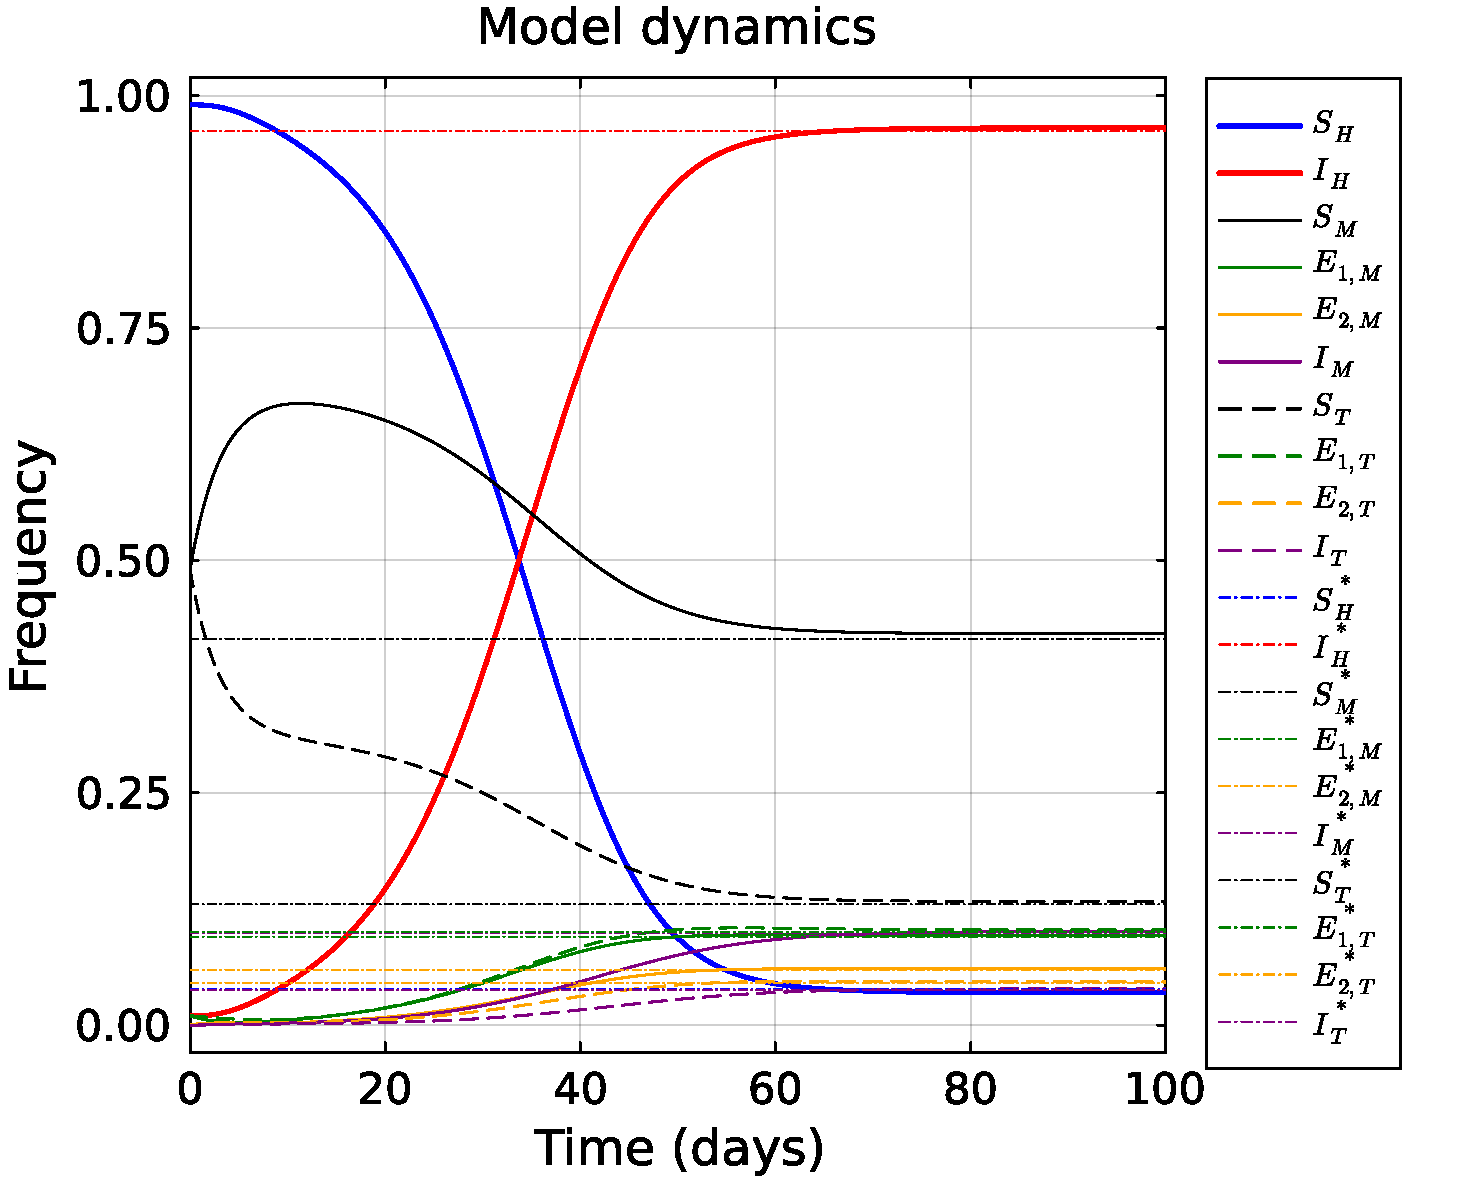
\includegraphics[width=0.65\textwidth]{../../fig/model_dynamics.pdf}
    \caption{Convergence to endemic equilibrium with default parameters. The EE is obtained from the symbolic expressions.}
\end{figure}

\subsection{Basic Reproduction Number}
\begin{figure}[H]
    \centering
    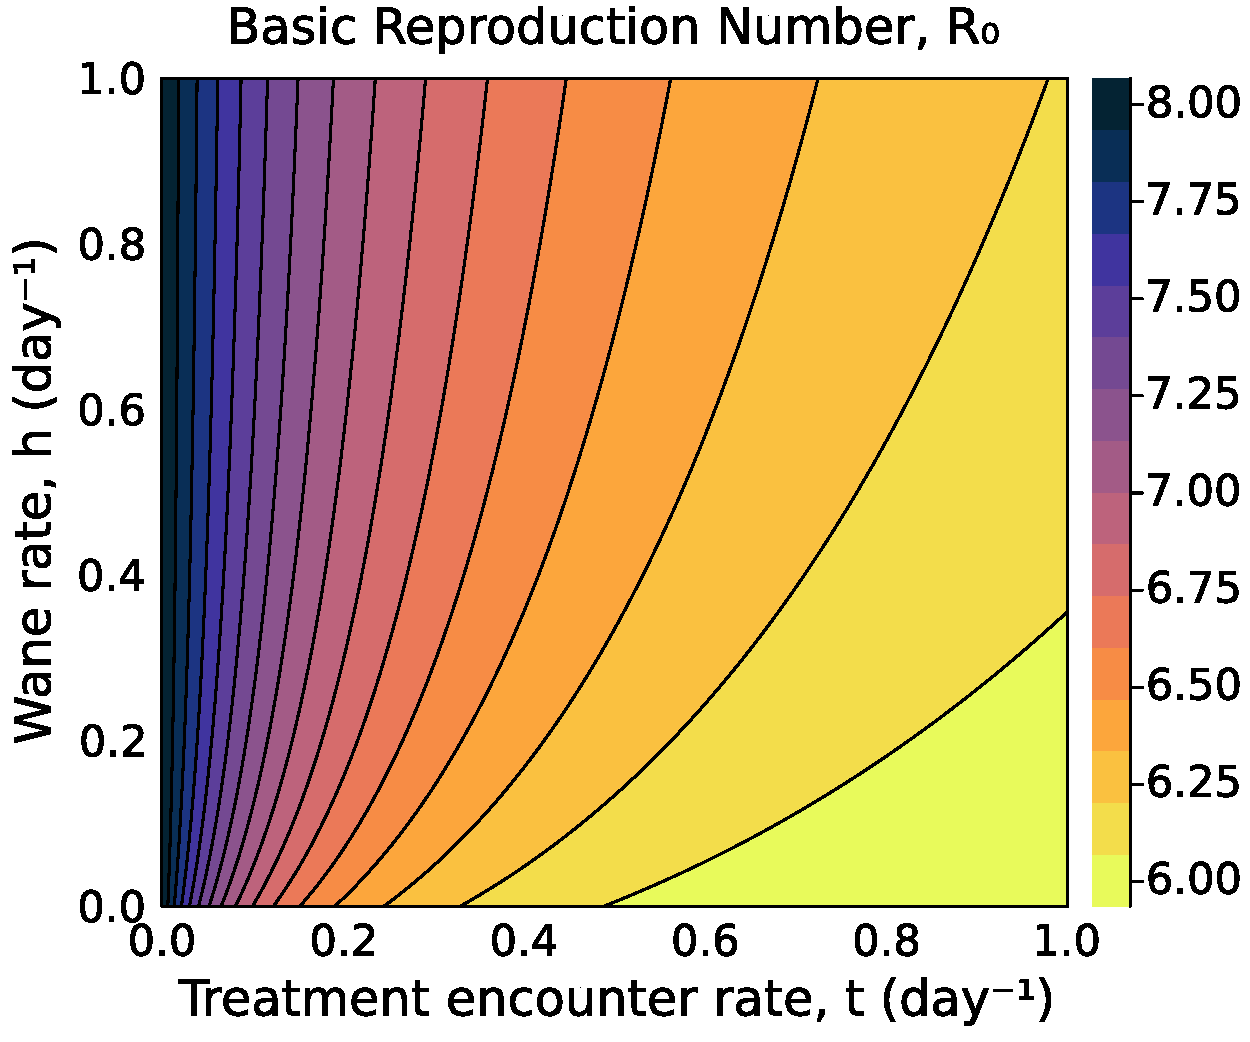
\includegraphics[width=0.49\textwidth]{../../fig/brn_txh_heatmap_m.pdf}
    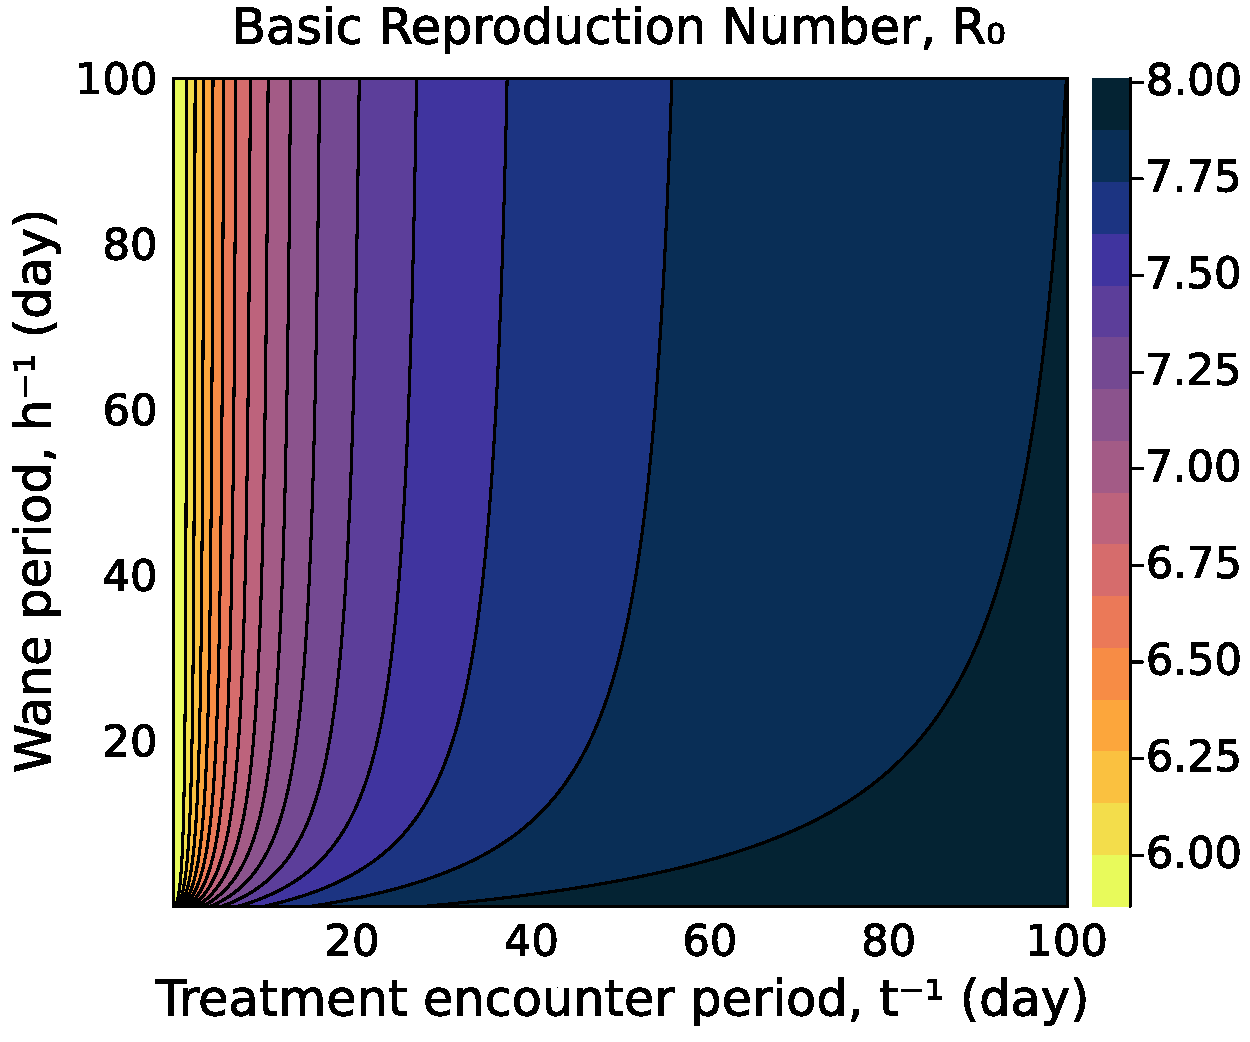
\includegraphics[width=0.49\textwidth]{../../fig/brn_txh_heatmap_rev_m.pdf}
    \caption{\(R_0\) vs treatment rates (\(t,h\)) and treatment periods (\(1/t,1/h\)). Results are obtained from the matrix method.}
\end{figure}

\begin{figure}[H]
    \centering
    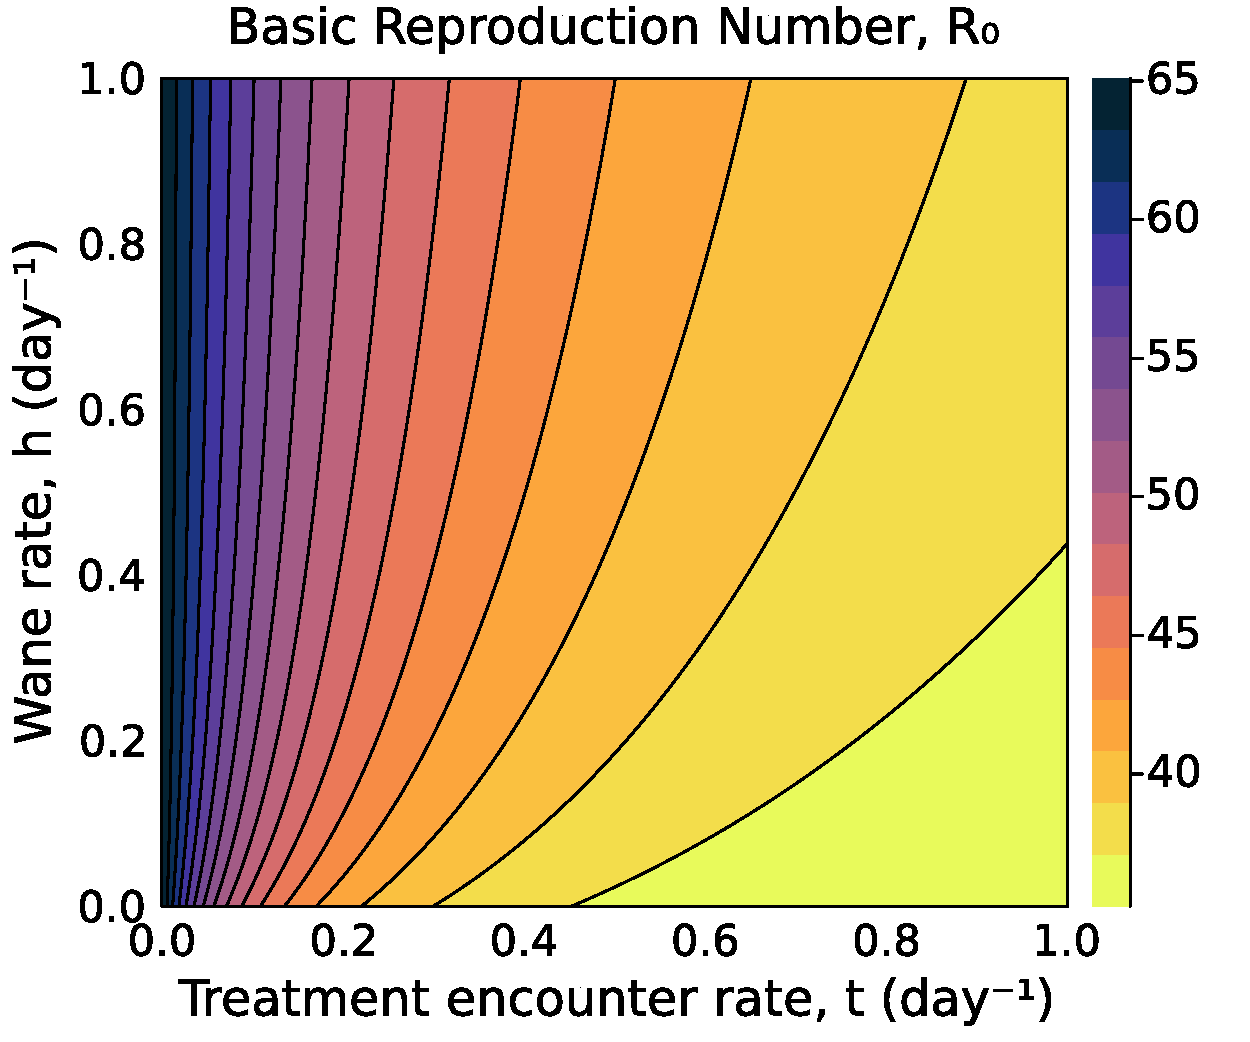
\includegraphics[width=0.49\textwidth]{../../fig/brn_txh_heatmap_s.pdf}
    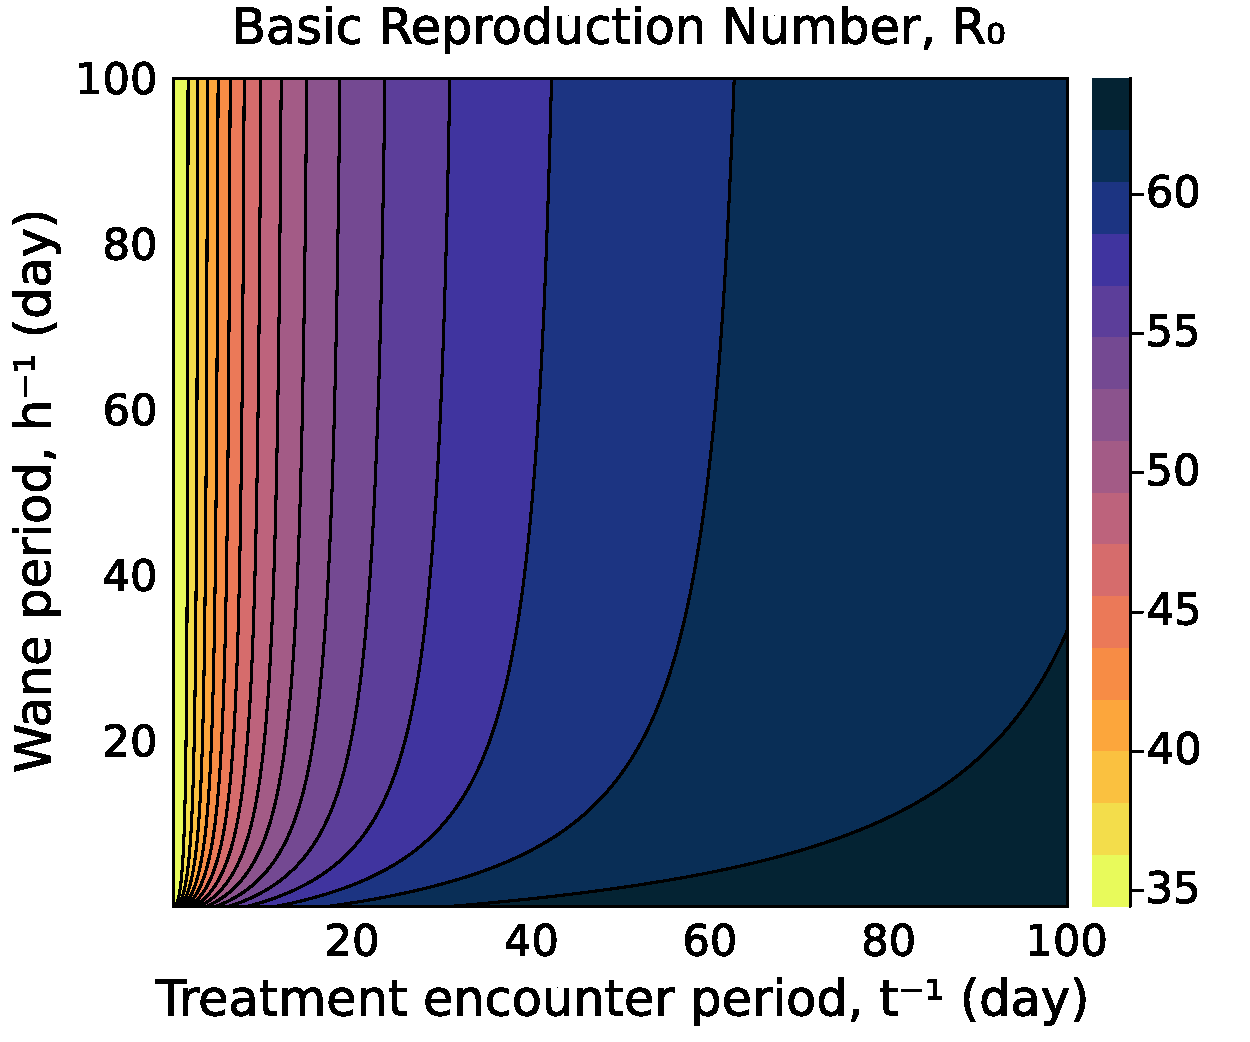
\includegraphics[width=0.49\textwidth]{../../fig/brn_txh_heatmap_rev_s.pdf}
    \caption{\(R_0\) vs treatment rates (\(t,h\)) and treatment periods (\(1/t,1/h\)). Results are obtained from the symbolic expressions.}
\end{figure}

\begin{figure}[H]
    \centering
    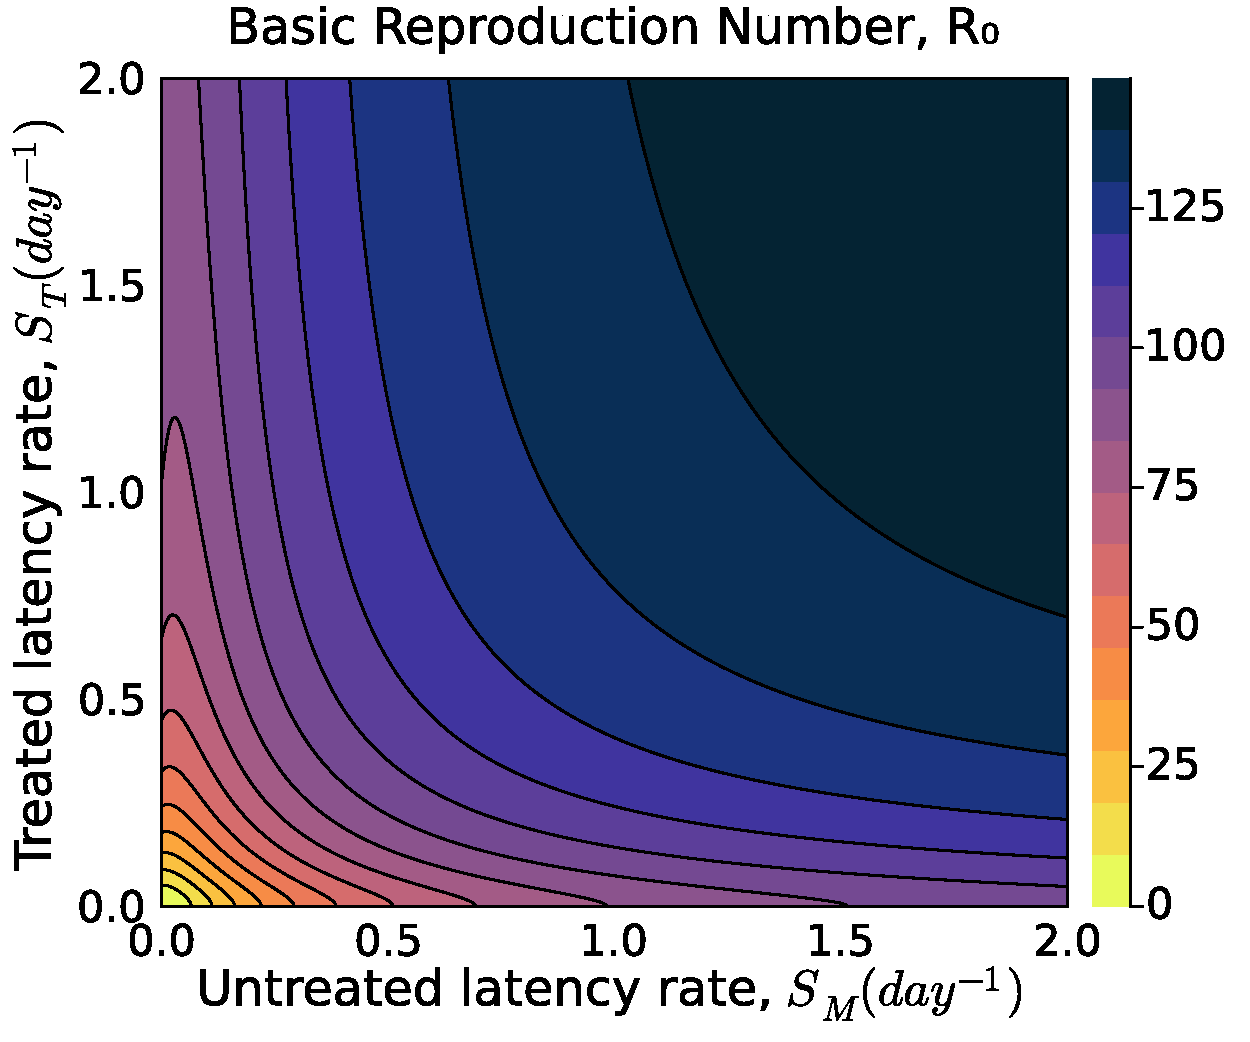
\includegraphics[width=0.49\textwidth]{../../fig/R0_STxSM.pdf}
    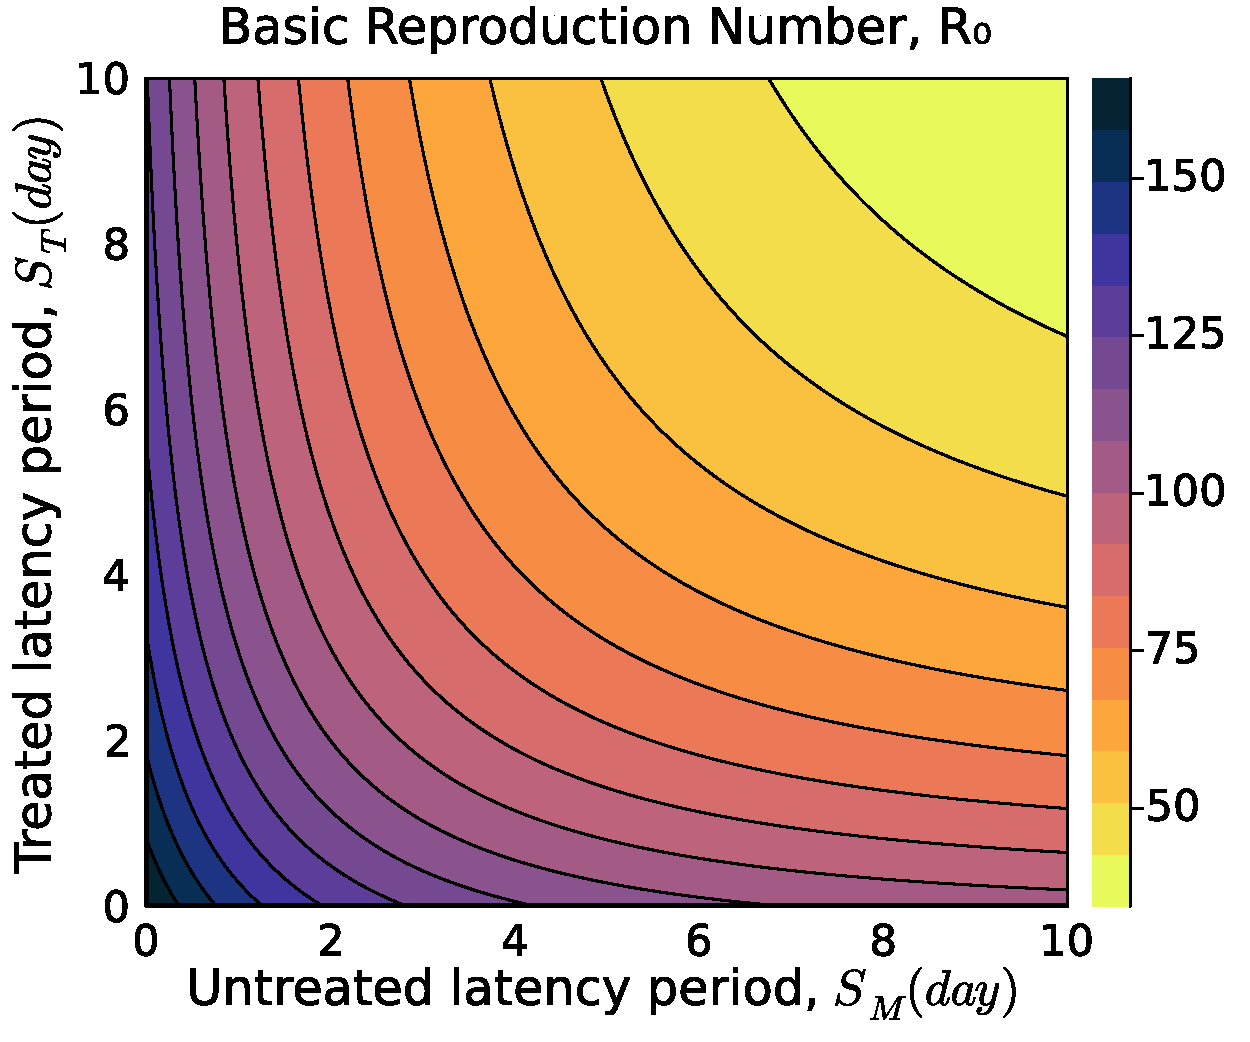
\includegraphics[width=0.49\textwidth]{../../fig/R0_STxSM_rev.pdf}
    \caption{\(R_0\) vs latency rates (\(s_{1M},s_{2M}\)) and treatment rates (\(s_{1T},s_{2T}\)). Results are obtained from the matrix method.}
\end{figure}

\begin{figure}[H]
    \centering
    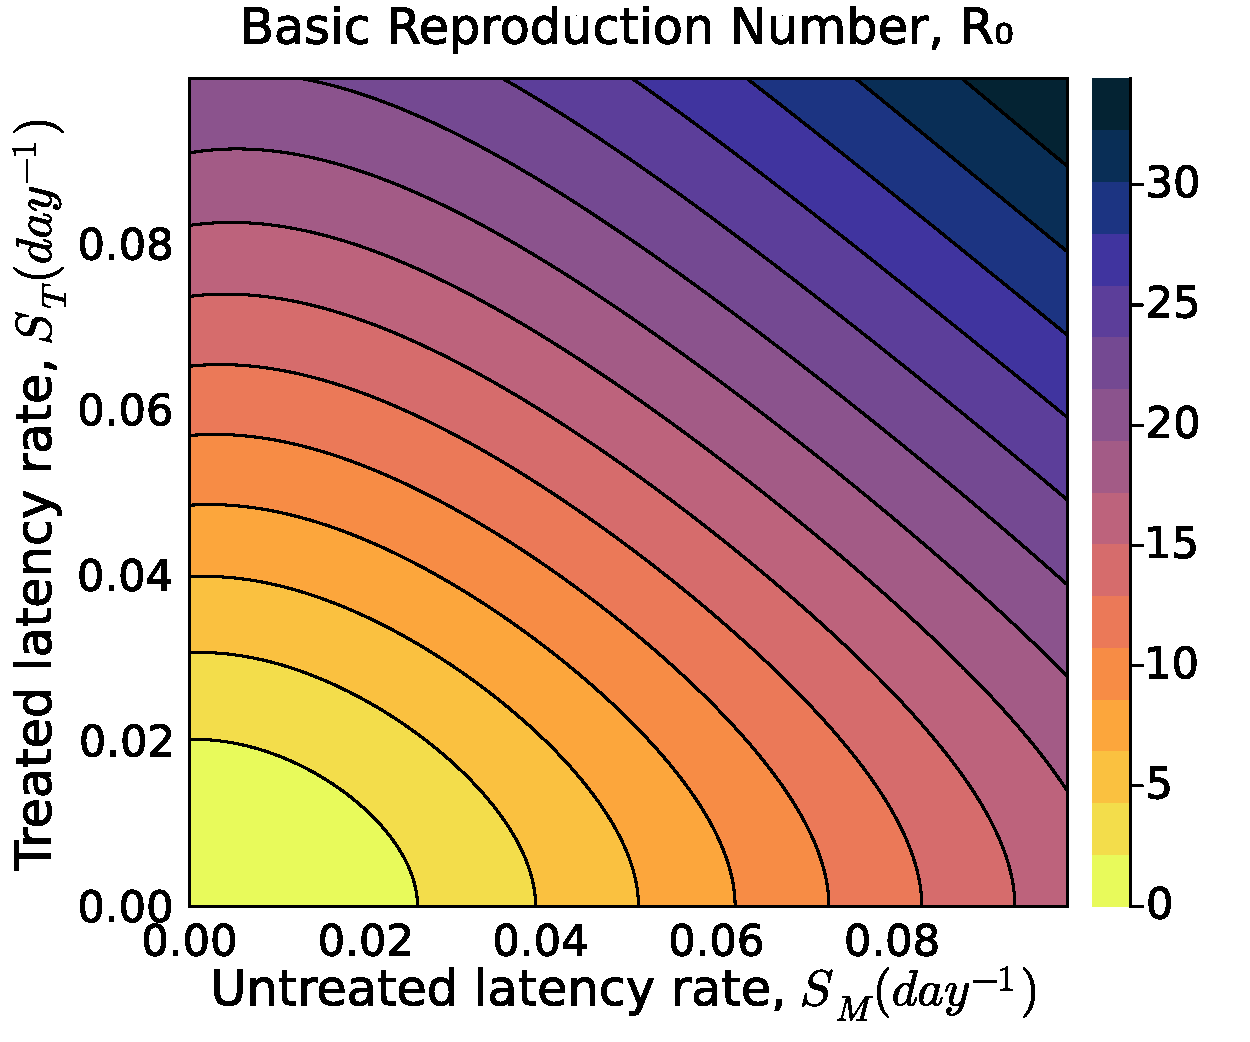
\includegraphics[width=0.49\textwidth]{../../fig/R0_STxSM_zoom.pdf}
    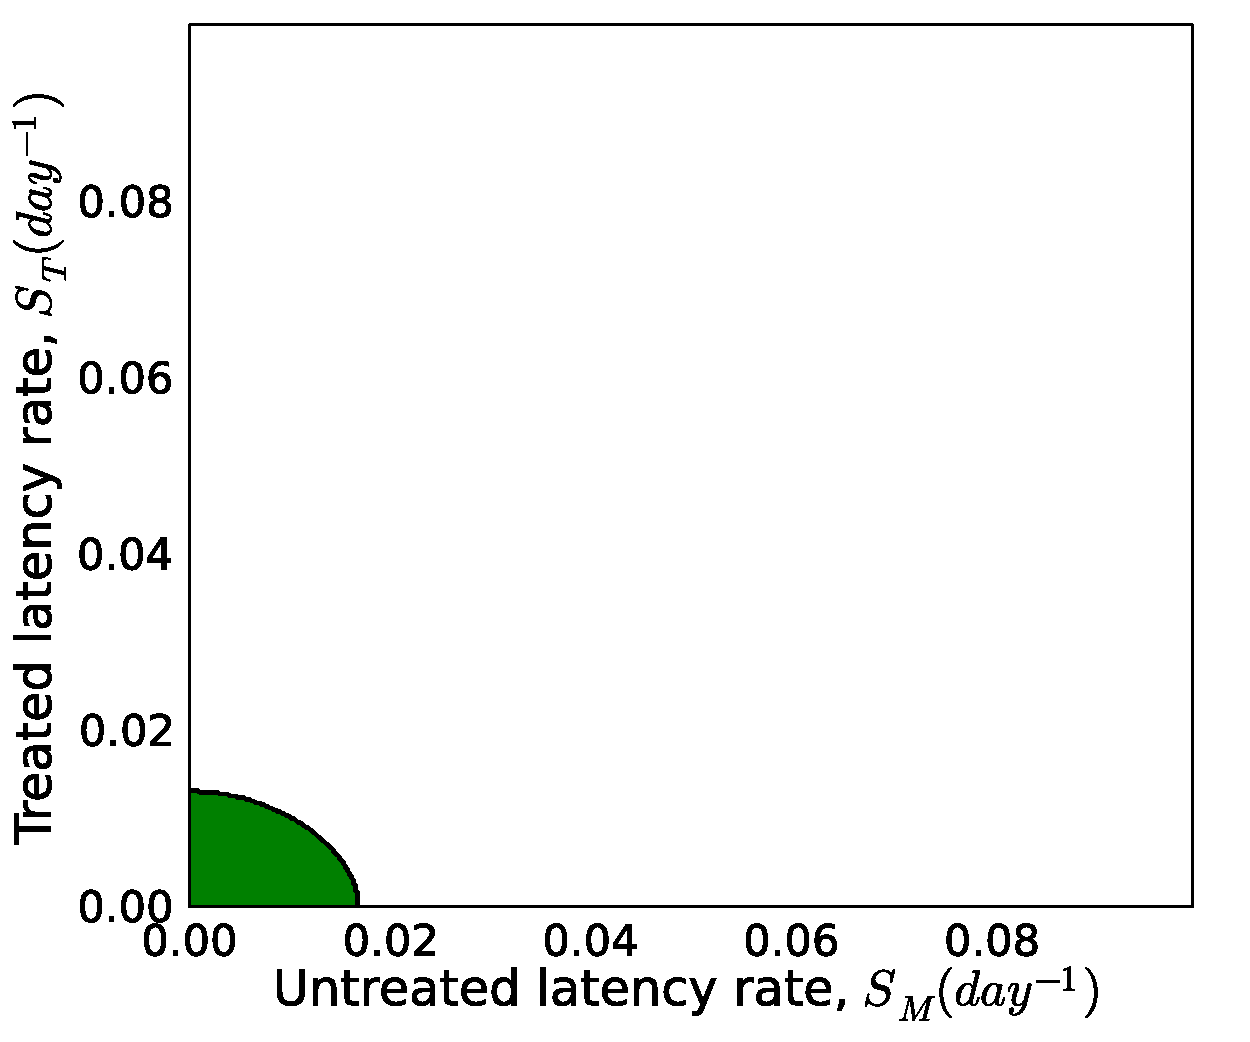
\includegraphics[width=0.49\textwidth]{../../fig/R0_STxSM_zoom_cut.pdf}
    \caption{\(R_0\) vs latency rates (\(s_{1M},s_{2M}\)) and $R_0 > 1$ cut. Results are obtained from the symbolic expressions.}
\end{figure}

\begin{figure}[H]
    \centering
    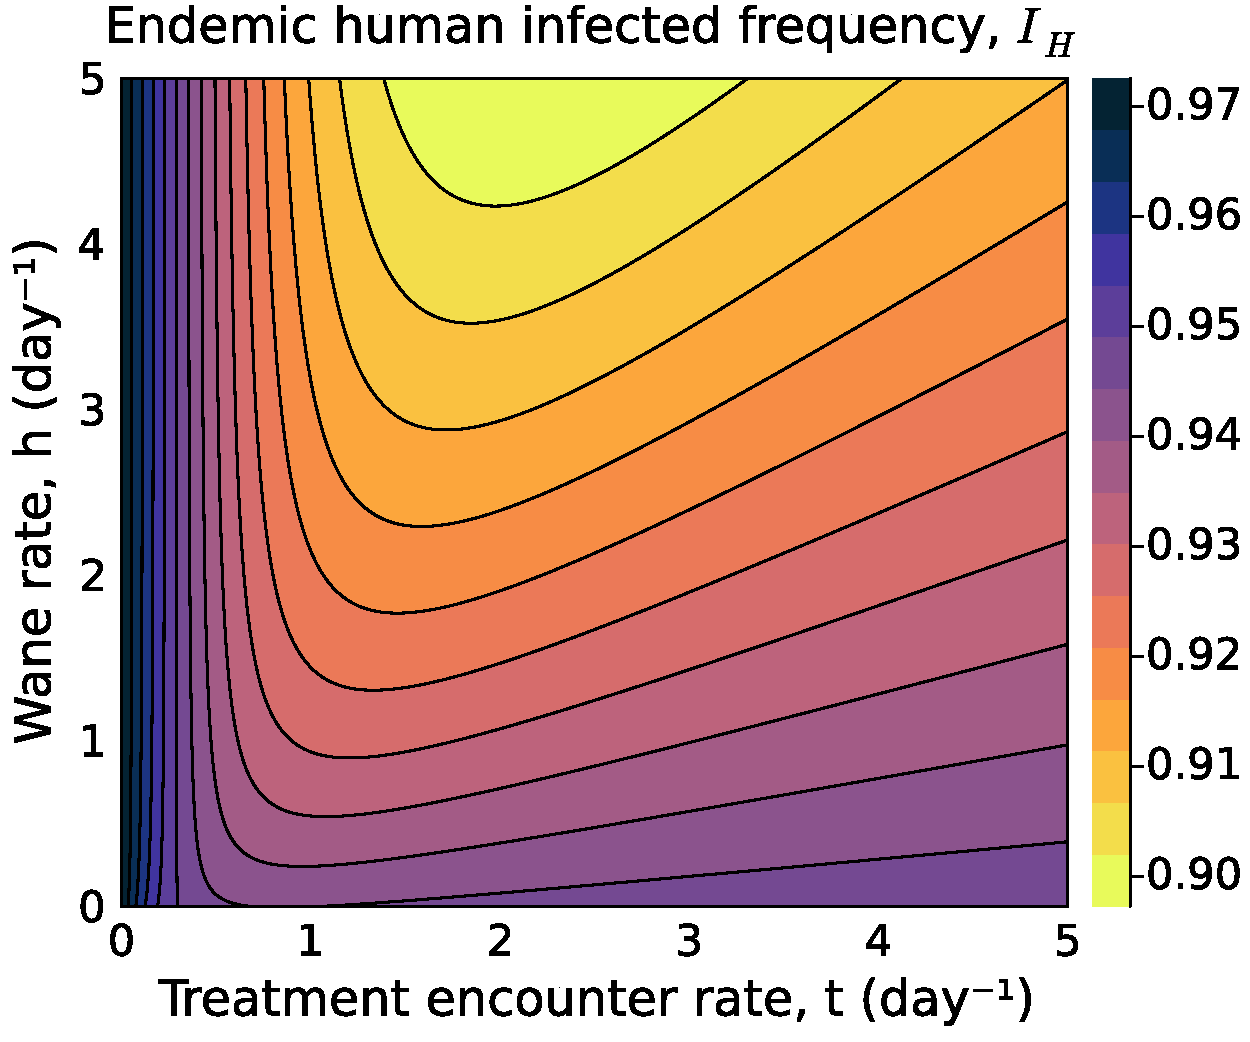
\includegraphics[width=0.49\textwidth]{../../fig/Ih_txh.pdf}
    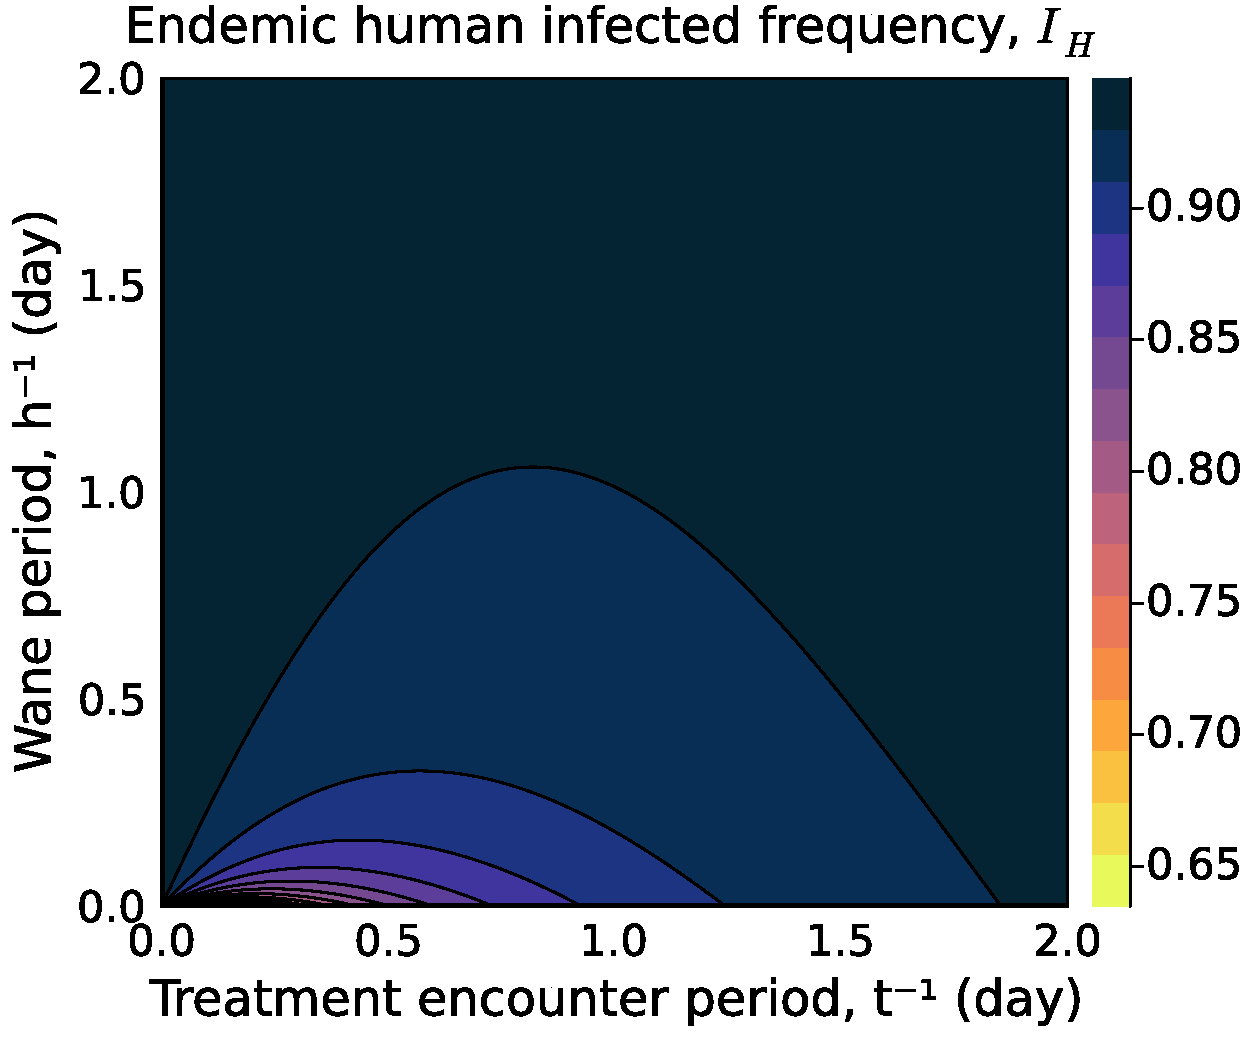
\includegraphics[width=0.49\textwidth]{../../fig/Ih_txh_rev.pdf}
    \caption{Endemic equilibrium of infections humans \(I_H^*\) vs treatment rates (\(t,h\)) and treatment periods (\(1/t,1/h\)). Results are obtained from the matrix method.}
\end{figure}

\begin{figure}[H]
    \centering
    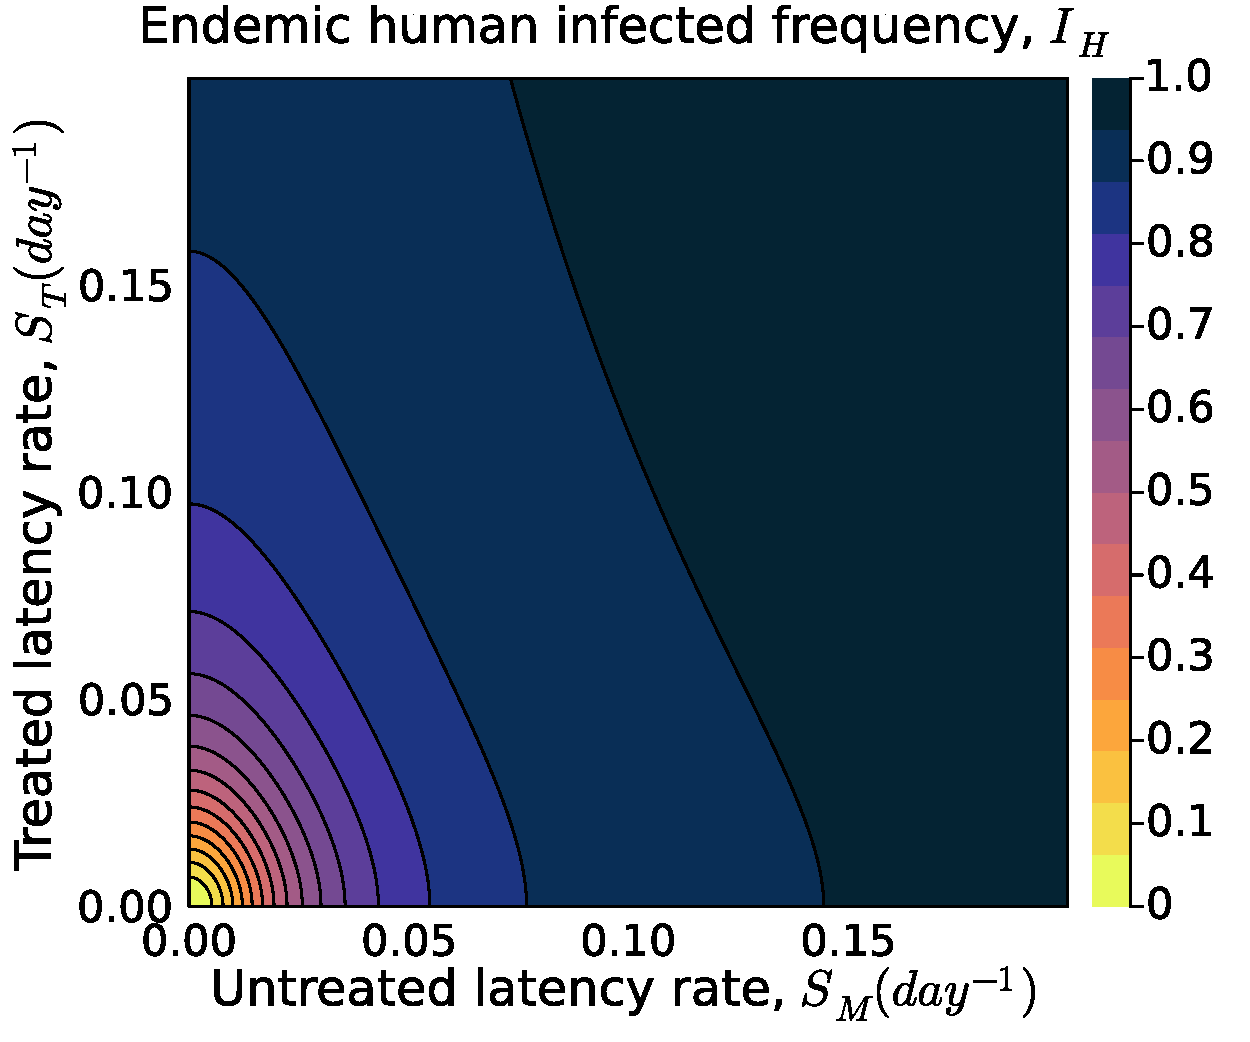
\includegraphics[width=0.49\textwidth]{../../fig/Ih_STxSM.pdf}
    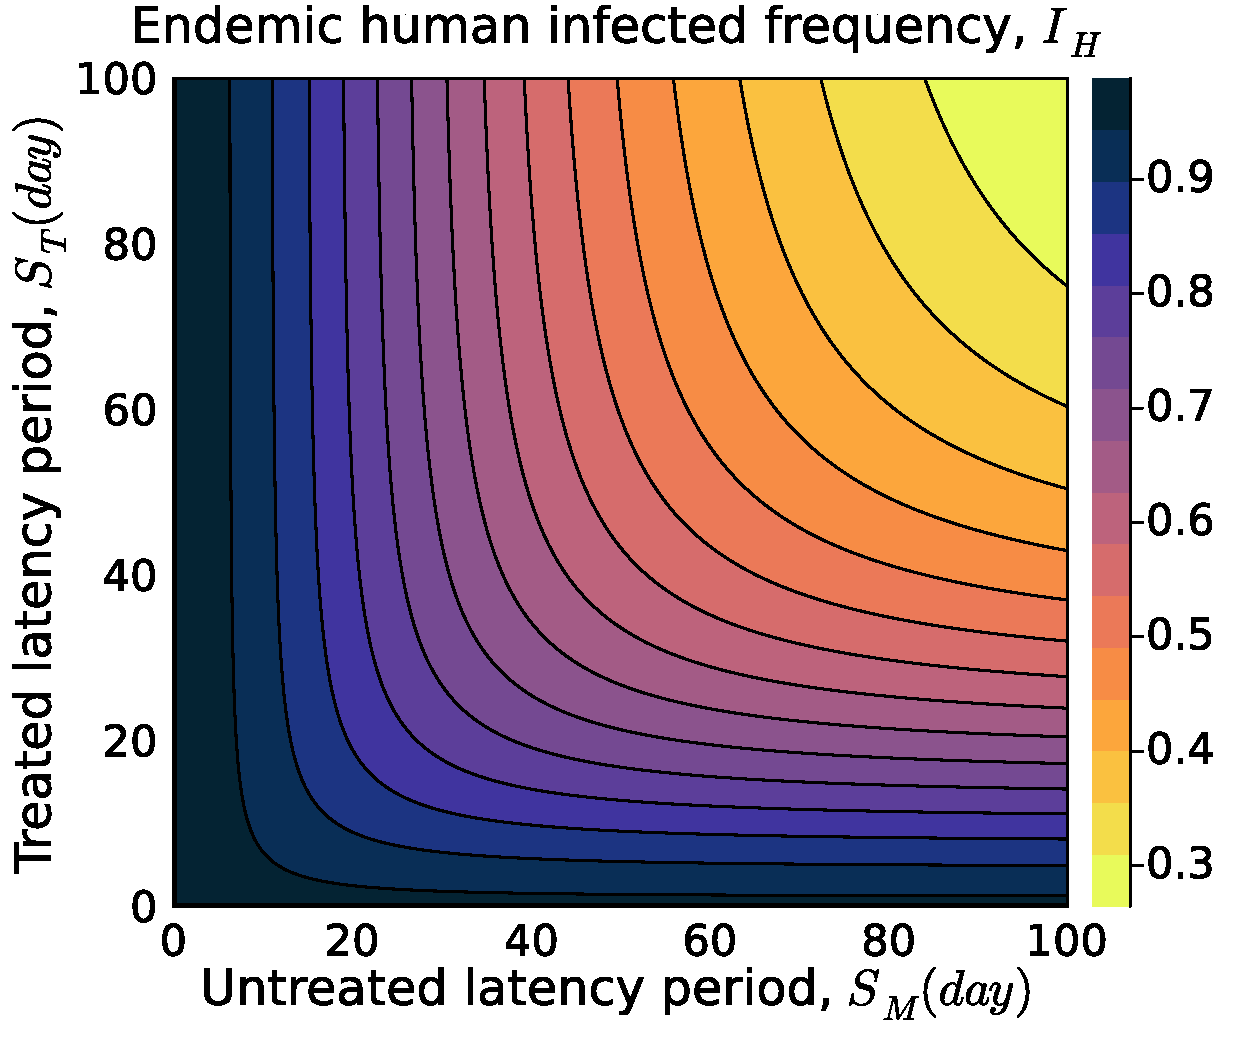
\includegraphics[width=0.49\textwidth]{../../fig/Ih_STxSM_rev.pdf}
    \caption{Endemic equilibrium of infections humans \(I_H^*\) vs latency rates (\(s_{1M},s_{2M}\)) and treatment rates (\(s_{1T},s_{2T}\)). Results are obtained from the matrix method.}
\end{figure}

\end{document}
